\myChapter{Service Oriented Architecture}\label{chap:soa}
\minitoc\mtcskip
\vfill
\lettrine{R}{esearch} in Service Oriented Architectures (SOA) \citep{PAPAZOGLOU} is an emerging field, as can be seen in Figure \ref{fig:soapapers}, obtained from the search terms {\em ``service oriented OR service-oriented''} in the Scopus \footnote{\url{http://www.scopus.com}} database. Each year more papers about the area are published. This area seeks to promote services usage and adoption, and to improve the way to use them. For example, solving a problem combining existing services in an automatic way \citep{COMPOSITION}.





\begin{SCfigure}[20][htb]
\centering
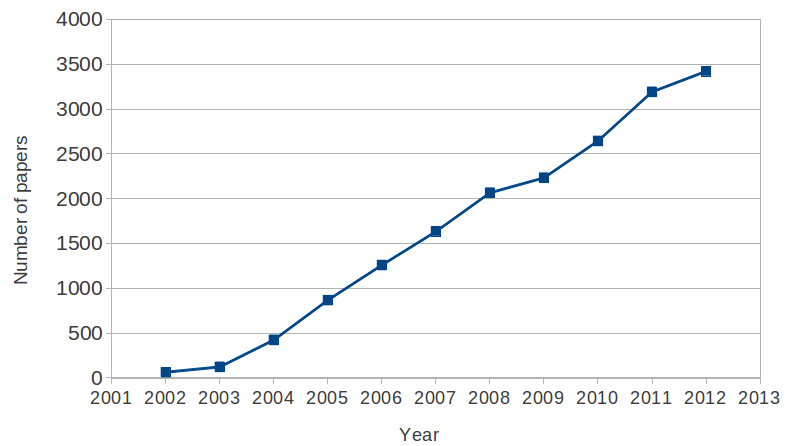
\includegraphics[width=26pc]{gfx/soa/papersYear.jpg}
\caption{Number of published papers (per year) about SOA (obtained from Scopus database).}
\label{fig:soapapers}
\end{SCfigure}


Service Oriented Architecture  is a computational
paradigm where the users interact with each other using the concept of
{\em service}. A service is a distributed entity (such as node, program,
function), used to obtain a result, increasing the integration of heterogeneous
systems (several operating systems, protocols or languages) due to
this multi-platform nature. The service users do not need to know
the language used to implement the service, and they are not
forced to use a specific technology to access that service. For
example, an evolutionary algorithms researcher could have access to a
fitness function made publicly available by another researcher at the
other side of the world without even knowing which programming language
has been used to implement it.



With the advancement of the Internet, new scientific communities, based on interoperable and distributed platforms are emerging. These communities allow scientist to collaborate in their research, sharing data and remote access to their programs. To achieve this, they use SOA, due to standards usage. Users publish and use flexible, interoperable and configurable services. These services can be created from scratch or by leveraging existing software. 

\cite{SERVICEORIENTEDSCIENCE05} defines the term ``Service Oriented
Science'' as the pursuit of scientific research using distributed and
interoperable networks, being the uniformity of
these interfaces the key to success. Thanks to it, researchers can discover and access
the services without developing specific access for each data source, or
program. Therefore, this paradigm has the potential to increase the
scientific productivity due to these public and distributed services, and also to increase the data analysis automation in computing. There are many examples that attempt to boost this paradigm, like Open Science Grid \citep{OPENSCIENCEGRID} and GLOBUS \citep{GLOBUS}. These projects are scientific communities and globally distributed infrastructures that support scientific and integrated applications of different domains.
It is necessary to remark that services implementation technology is not the
great challenge in SOA (neither the specific technology presented in
this work).
Its main goal is to increase the effort to migrate the
existing work and to change the mind of researchers and
practitioners. 

\begin{SCfigure}[20][htb]
\centering
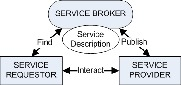
\includegraphics[width=26pc]{gfx/soa/soaDiagram.jpg}
\caption{Service interaction schema. The service provider publishes a service description that is used by the consumer to find and use the service.}
\label{fig:soadiagram}
\end{SCfigure}


Figure \ref{soadiagram} shows the basic interaction among
services. First, the {\em service provider} exposes the service, publishing
its interface in the {\em service broker}. The {\em service consumer} (or
{\em requestor}) finds in the broker a service to be used and receives its
interface. Then the request is performed by the {\em consumer} (which uses or
consumes the service).  

Moreover, several implementations of a specific service  can exist (in one or several machines). The broker can choose which one to use  each time, or offer another if a service is unavailable. Implementations  may also have a different behavior, so the researcher can take advantage to create an auto-adaptive algorithm to select different implementations according to some criteria. Figure \ref{SERVICEBASIC} shows this special interaction, where two different implementations of an operator interface exist (even using different languages) and the broker has chosen one of them.


The service broker in a SOA can be implemented in several ways and have
different behaviors: for example, the implementations of the services to be used can be
defined in a text file (if the services do not change in execution
time). However, the broker can also assign implementations to
interfaces in an automatic way, or using several rules, for example,
to distribute a fitness between several machines activated while the
algorithm is running. 


\begin{SCfigure}[20][htb]
\centering
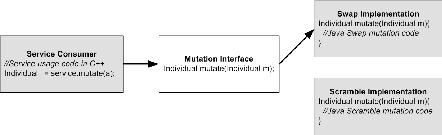
\includegraphics[width=26pc]{gfx/soa/serviceEA.jpg}
\caption{Example of usage of a service implementation.}
\label{SERVICEBASIC}
\end{SCfigure}




An important SOA capability is that it is not focused on a specific
implementation, but offers a set of guidelines to help the
developers. In \citep{SOMA} these guidelines and good practices, and also the differences between SOA and Object Oriented
Programming (OOP) are
explained: the main difference between SOA and imperative programming or OOP is the order of service execution. This order is not necessarily static, because the services are designed to be used in a non-established and configurable order. Furthermore, another important difference is that services can be dynamically discovered and used (while in OOP must be previously known and can not change during execution), being also one of the most important capabilities the (optional) distribution in a network. Finally, in OOP the programming language must be the same for each method call.

\section{Implementation technologies}

\subsection{SOAP, WSDL and BPEL}

\subsection{OSGi}
OSGi, was proposed by a consortium of more than
eighty companies in order to develop an infrastructure for the
deployment of service in heterogeneous network of devices, mainly
oriented to domotics \cite{GATEWAY}. Nowadays it defines a
specification for a Service Oriented Architecture for virtual
machines (VMs). It provides very desiderable features, like
packet abstraction, life-cycle management, packaging or versioning,
allowing significant reduction of the building, support and deployment
complexity of the applications. 

OSGi technology allows dynamic discovery of new components, to increase the collaboration and to minimize and manage the coupling
among modules. Moreover, the
OSGi Alliance has developed several standard component interfaces for
common usage patterns, like HTTP servers, configuration, logs, security,
management or XML management among others, whose implementations can
be obtained by third-parties. Nowadays there are some challenges 
in the OSGi development \cite{OSGICHALLENGES}, but they only affect the creation of very complex applications.

This advantages are not so
                               costly, as can be thought: the OSGi
                                framework can be implemented in a
                                {\em jar} file\footnote{A jar file is
                                a file that groups the compiled Java
                                files.} of 300KB. Also, and different
                                of the normal usage of Java, each
                                class pre-charges only the other
                                classes to use, not all. Also is
                                non-intrusive: the code to be
                                executed in OSGi can be executed
                                without it. Finally, from its
                                specification in 1998 has been widely
                                used as base in big projects: the
                                Eclipse IDE (Integrated Development
                                Environment) is built over OSGi, and
                                also big application servers
                               (Glassfish or IBM Websphere) or
                               residential gateways
                               \cite{GATEWAY}, among other
                               examples. 

\subsection{OSGi Architecture}
To understand how OSGi \cite{OSGI} works and which capabilities could offer to the OSGiLiath users it is necessary to understand how OSGi is built. OSGi has a layered model that is depicted in Figure \ref{fig:osgi-original}. The terms present in this Figure are:

\begin{itemize}
\item Bundles: Bundles are the OSGi components made by developers. Is a normal {\em jar} file including Java classes and interfaces with different MANIFEST.MF and extra files (such as the Service Descriptions).
\item Services: This layer connects bundles in a dynamic way by offering a publish-find-bind model.
\item Life-Cycle: The API to install, start, stop, update, and uninstall bundles.
\item Modules: This layer defines how a bundle can import and export code (using the MANIFEST.MF file).
\item Security: Security aspects are handled in this layer.
\item Execution Environment: Defines what methods and classes are available in a specific platform. For example, mobile devices have less Java classes due to performance constraints.
\end{itemize}

\begin{SCfigure}[20][htb]
\centering
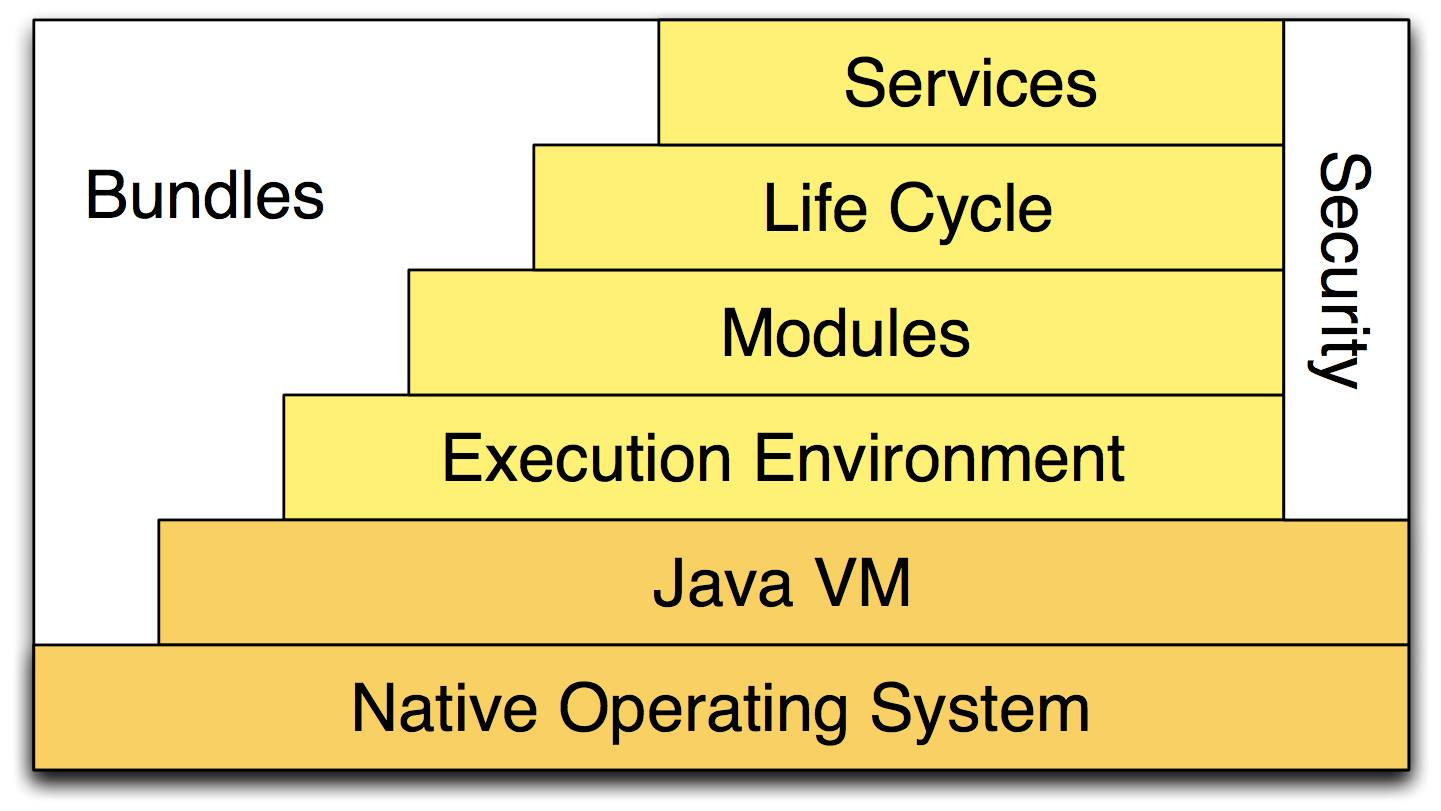
\includegraphics[width=26pc]{gfx/soa/osgi-oficial.jpg}
\caption{OSGi layered architecture. Every layer is built from the one just below.}
\label{fig:osgi-original}
\end{SCfigure}






\subsection{OSGi configuration files}
Regarding to explained OSGi layers how to use all OSGi capabilities is shown next. 

OSGi implements a dynamic component model, unlike normal Java
environments. Applications or components (also called
\emph{bundles}) can be remotely installed, started, stopped, updated
or uninstalled on the fly; moreover, the classes and
packaging management is specified in detail. The OSGi framework provides
APIs for the management of services that are exposed or used by the
bundles.

Java programmers are familiar with the {\em jar} concept. The first difference among a {\em bundle} and a {\em jar} is that the second has a MANIFEST.MF file adapted to be used in OSGi. This file indicates which clases imports or exports the {\em bundle}. An example can be seen in Figure \ref{fig:manifest}. This file shows the name of the bundle and its version (this is useful to select specific services), and the execution environment (that is, the Java Virtual Machine required). Also, this file specifies the XML files of the declarative services (in section {\em Service-Component}). However, this {\em bundle} can be used as a normal {\em jar} outside OSGi.

\begin{figure}[t]
\noindent
\ttfamily
\hlstd{}{\bf Manifest-Version:} 1.0\\
\hlstd{}{\bf Bundle-ManifestVersion:} 2\\
\hlstd{}{\bf Bundle-Name:} VRP\\
\hlstd{}{\bf Bundle-SymbolicName:} VRP\\
\hlstd{}{\bf Bundle-Version:} 1.0.0\\
\hlstd{}{\bf Bundle-RequiredExecutionEnvironment:} JAVA-1.6\\
\hlstd{}{\bf Import-Package:}  es.ugr.osgiliath,\\
 \hlstd{}  es.ugr.osgiliath.algorithms,\\
\hlstd{} es.ugr.osgiliath.events,\\
 \hlstd{}es.ugr.osgiliath.evolutionary,\\
 \hlstd{}es.ugr.osgiliath.evolutionary.basiccomponents.genomes,\\
 \hlstd{}es.ugr.osgiliath.evolutionary.basiccomponents.individuals,\\
 \hlstd{}es.ugr.osgiliath.evolutionary.elements,\\
 \hlstd{}es.ugr.osgiliath.evolutionary.individual,\\
 \hlstd{}es.ugr.osgiliath.evolutionary.migrator,\\
 \hlstd{}es.ugr.osgiliath.geneticalgorithm.distributed,\\
 \hlstd{}es.ugr.osgiliath.problem\\
\hlstd{}{\bf Export-Package:} es.ugr.osgiliath.vrp,\\
 \hlstd{}es.ugr.osgiliath.vrp.individual\\
\hlstd{}\hlkwa{Service-Component:} OSGI-INF/vrpinitializer.xml,\\
OSGI-INF/vrpfitnesscalculator.xml,\\
 OSGI-INF/vrpcrossover.xml,\\
 OSGI-INF/vrpmutation.xml\\
\mbox{}
 
\normalfont
\caption{Example of MANIFEST.MF. This example defines which packages are necessary to activate the bundle and which packages are exported.}
\label{fig:manifest}
\end {figure}





In normal environments, to create a specific implementation of an interface (i.e. {\em FitnessCalculator}) is as follows:

\begin{lstlisting}
class EvolutionaryAlgorithm implements Algorithm{
 FitnessCalculator fc;
 //A new instance is bound to a reference
 fc = new ExampleFunction();
}
\end{lstlisting}
 
With Declarative Services, the {\em new ExampleFunction()} part is not used, so if a new implementation is desired no code recompilation is necessary.  Figure \ref{fig:ds} shows a declarative service description file, which establish in execution time which implementation is bound to the interfaces. This example indicates that the implementation of service {\em FitnessCalculator} is {\em VRPFitnessCalculator}, but this service is not activated until all their references (other services, like {\em TransportData}) are also activated. The tag {\em cardinality} means that at least one service of that kind must exist (the first {\em 1} represents optionality) and  the second part (the other {\em 1} indicates the number of different implementations that can be managed: one ({\em 1}) or many ({\em *}).  We need to create XML files for the rest of services to expose (i.e. {\em TransportData}). The file where these capabilities are defined is declared in section {\em Service-Component} of MANIFEST.MF file, as can be seen in Figure \ref{fig:manifest}.
\begin{figure*}[t]
\noindent
\ttfamily
\hlstd{}\hlopt{$<$}\hlstd{?xml\ version}\hlopt{=}\hlstd{"}\hlnum{1.0}\hlstd{"\ encoding}\hlopt{=}\hlstd{"UTF{-}8"?}\hlopt{$>$}\hspace*{\fill}\\
\hlstd{}\hlopt{$<$}\hlstd{scr}\hlopt{:}\hlstd{component\ xmlns}\hlopt{:}\hlstd{scr}\hlopt{=}\hlstd{"http}\hlopt{://}\hlstd{www}\hlopt{.}\hlstd{osgi}\hlopt{.}\hlstd{org}\hlopt{/}\hlstd{xmlns}\hlopt{/}\hlstd{scr}\hlopt{/}\hlstd{v1}\hlopt{.}\hlstd{1}\hlnum{.0}\hlstd{"\ name}\hlopt{=}\hlstd{"VRPFitnessCalculator"}\hlopt{$>$}\hspace*{\fill}\\
\hlstd{}\hlstd{\ \ \ }\hlstd{}\hlopt{$<$}\hlstd{implementation\ class}\hlopt{=}\hlstd{"es}\hlopt{.}\hlstd{ugr}\hlopt{.}\hlstd{osgiliath}\hlopt{.}\hlstd{vrp}\hlopt{.}\hlstd{VRPFitnessCalculator"}\hlopt{/$>$}\hspace*{\fill}\\
\hlstd{}\hlstd{\ \ \ }\hlstd{}\hlopt{$<$}\hlstd{service}\hlopt{$>$}\hspace*{\fill}\\
\hlstd{}\hlstd{\ \ \ \ \ \ }\hlstd{}\hlopt{$<$}\hlstd{}\hlkwa{provide\ }\hlstd{interface}\hlopt{=}\hlstd{"es}\hlopt{.}\hlstd{ugr}\hlopt{.}\hlstd{osgiliath}\hlopt{.}\hlstd{evolutionary}\hlopt{.}\hlstd{elements}\hlopt{.}\hlstd{FitnessCalculator"}\hlopt{/$>$}\hspace*{\fill}\\
\hlstd{}\hlstd{\ \ \ }\hlstd{}\hlopt{$<$/}\hlstd{service}\hlopt{$>$}\hspace*{\fill}\\
\hlstd{}\hlstd{\ \ \ }\hlstd{}\hlopt{$<$}\hlstd{reference\ bind}\hlopt{=}\hlstd{"setTransportData"\ \hspace*{\fill}\\
}\hlstd{\ \ \ \ }\hlstd{unbind}\hlopt{=}\hlstd{"unsetTransportData"\hspace*{\fill}\\
}\hlstd{\ \ \ \ }\hlstd{cardinality}\hlopt{=}\hlstd{"}\hlnum{1}\hlstd{}\hlopt{.}\hlstd{}\hlnum{.1}\hlstd{"\ \hspace*{\fill}\\
}\hlstd{\ \ \ \ }\hlstd{interface}\hlopt{=}\hlstd{"es}\hlopt{.}\hlstd{ugr}\hlopt{.}\hlstd{osgiliath}\hlopt{.}\hlstd{vrp}\hlopt{.}\hlstd{TransportData"\ \hspace*{\fill}\\
}\hlstd{\ \ \ \ }\hlstd{name}\hlopt{=}\hlstd{"TransportData"\ \hspace*{\fill}\\
}\hlstd{\ \ \ \ }\hlstd{policy}\hlopt{=}\hlstd{"static"\hspace*{\fill}\\
}\hlstd{\ \ \ }\hlstd{}\hlopt{/$>$}\hspace*{\fill}\\
\hlstd{}\hlstd{\ \ \ }\hlstd{}\hlopt{$<$}\hlstd{property\ name}\hlopt{=}\hlstd{"name"\ }\hlkwa{type}\hlstd{}\hlopt{=}\hlstd{"String"\ }\hlkwa{value}\hlstd{}\hlopt{=}\hlstd{"vrpfitnesscalculator"}\hlopt{/$>$}\hspace*{\fill}\\
\hlstd{}\hlopt{$<$/}\hlstd{scr}\hlopt{:}\hlstd{component}\hlopt{$>$}\hlstd{}\hspace*{\fill}\\
\mbox{}
\normalfont
\caption{Service Description. This documents indicates that the implementation of the service {\em FitnessCalculator} is {\em VRPFitnessCalculator}, but it can not activate until their references (other services) are activated.}
\label{fig:ds}
\end {figure*}

 Next code shows the code for this implementation:

\begin{lstlisting}
class VRPFitnessCalculator implements FitnessCalculator{
 //Other service references,
 TransportData tdata;
 
 //Methods to bind/unbind each reference
 public TransportData 
    setTransportData(TransportData tdata){
  this.tdata = tdata;
 }
	
 public void 
    unsetTransportData(TransportData tdata){
  this.tdata = null;
 }

 //Implementation of the interface method
 List<Fitness> calculateFitness(List<Individual> inds){
 	...
 }
}
\end{lstlisting}

%We have to say that in future work these kind of files will be automatically created, being this task transparent to future users of the OSGiLiatH framework.

\subsection{Event Administration}
The Event Administration in OSGi lets the usage of a blackboard communitacion architecture where bundles can broadcast or receive events without notice which bundles are sending or receiving these events.

%Acquire a reference to the EventAdmin OSGi service, it implements the org.osgi.service.event.EventAdmin.
%Pick a topic name for the event and make sure that it follows Topic Naming Conventions mentioned above.
%Fill Event Properties in a dictionary that will be passed as a parameter to the publish method.
%Having the Topic Name and Properties, ready invoke one of the following methods of the Event Admin service: postEvent or sendEvent - while postEvent initiates synchronous delivery of the event, sendEvent initiates asynchronous delivery of the event. So by default, your option should be postEvent method unless you have strict requirements to not continue execution until all handlers of the event handle it.

To send events to other bundles:
\begin{itemize}
\item Acquire a reference to the EventAdmin OSGi service (via Declarative Services, for example).
\item Pick a topic name for the event (for example {\em ``es/ugr/osgiliath/algorithms/endgeneration''})
\item Send the event using the {\em postEvent} method of EventAdmin, with the topic plus other desired properties %(poner lo de sincrono/asincrono?)
\end{itemize}

Code to send an event to other bundles is shown below. The programmer specifies the topic String and optional properties to send to other bundles that are listening. The {\em eventAdmin} variable is a reference to {\em ``org.osgi.service.event. EventAdmin''} service, obtained via Declarative Services or by hand (not showed).

\begin{lstlisting}
Properties props = new Properties(); //Optional
String topic = 
   "es/ugr/osgiliath/algorithms/endgeneration";
Event evt = new Event(topic,props);
eventAdmin.postEvent(evt);
\end{lstlisting}
		
For the other hand, the steps to handle events are:
\begin{itemize}
\item Register a service that implements the OSGi EventHandler interface (via Declarative Services or manually).
\item Specify in this service the topics to subscribe to. For example, the String {\em ``es/ugr/osgiliath/algorithms/*''} (the * is a wildcard) inside the $<$property$>$ tag in the Service Description.
\item Overwrite the handleEvent method of this interface with the desired code.
\end{itemize}

This code shows how to handle events. In this case we have published the {\em ExampleService} with the implementation {\em ExampleImpl}, that is listening under the topic {\em ``es/ugr/osgiliath/algorithms/*''}.

\begin{lstlisting}
class ExmplImpl implements ExmplService,EventHandler{

 public void handleEvent(Event ev){
  if(evt.getTopic().endsWith("endgeneration")){
   // An event with topic 
   // "es/ugr/osgiliath/algorithms
   // /endgeneration"
   System.out.println("Generation over");
  else{
   // Other event with topic starts with
   // "es/ugr/osgiliath/algorithms/"
   System.out.println("Other event received");
  }
 }
}
\end{lstlisting}

%%%%%%%%%%%%%%%%%%  DEVELOPMENT  %%%%%%%%%%%%%%%%%%%

\subsection{Distribution}
In a good service-oriented framework for EAs all services must be capable to be indistinguishable of being a local or a remote service. Services can be distributed using the OSGi features. In this case, the distribution is performed using the service descriptor to set which service is distributable and which is the distribution technology that provides service discovering and data transmission.

OSGi allows several implementations for the service distribution. ECF (Eclipse Communication Framework)\footnote{\url{http://www.eclipse.org/ecf/}} has been chosen because it is the most mature and accepted implementation \cite{petzold2011dynamic}, and it also supports the largest number of transmission protocols, including both synchronous and asynchronous communication. It provides a modular implementation of the OSGi 4.2 Remote Services standard\footnote{\url{http://www.osgi.org/Release4/Download}}. This specification uses the OSGi service registry to expose remote services to other machines (being indistinguishable from the local ones). ECF also separates the source code from the discovery and transmission mechanism, allowing users to apply the most adequate technology to their needs, and providing the integration with existing applications. % For example, the lines of Figure \ref{fig:remote} have been added to the service descriptor of {\em MOP2 Fitness Calculator} to distribute it in the local network.

ECF includes a number of protocols for service discovery and service providers:
\begin{itemize}
\item Service Discovery API: Includes protocols to announce and discover remote services: Zeroconf, SLP/RFC 2608, Zookeeper, file-based and others \footnote{\url{http://wiki.eclipse.org/ECF_API_Docs\#Discovery_API}}.
\item Remote Service API: Includes protocols to establish the communication (data streams, formats and others): R-OSGi, ActiveMQ/JMS, REST, SOAP, XMPP, ECF Generic \footnote{\url{http://wiki.eclipse.org/ECF_API_Docs\#Remote_Services_API}}. This allow to communicate to systems that do not use OSGi or Java.
\end{itemize}